\chapter{Generazione schema da netlist}

Durante lo sviluppo di sistemi CAD per il disegno di circuiti elettrici, la compatibilità con formati di ingresso presenti sul panorama attuale rappresenta un fattore di flessibilità molto importante. Può risultare utile la lettura di file generati da software simili ma aventi caratteristiche diverse, come ad esempio risolutori numerici e simbolici o anche solo risolutori di generazioni successive. Non tutti i formati, però, recano con sé informazioni riguardanti la dislocazione grafica dei componenti all'interno di uno spazio di disegno, addirittura spesso il problema è dato dal fatto che dati riguardanti la struttura del circuito e la sua rappresentazione grafica sono suddivisi in file diversi.

Basti pensare ad esempio alle \textit{netlist} prodotte come formato intermedio da SapWin \cite{sapwin}, di cui un esempio è riportato nel listato \ref{netlist} dove è descritto il modello relativo ad un amplificatore operazionale. Di fatto le informazioni presenti indicano i nodi ai quali il componente si aggancia, il suo valore numerico e il suo stato (se deve essere cioè trattato effettivamente come valore numerico o come componente simbolico). Niente di tutto ciò, intuitivamente, può aiutare nella generazione di uno schema.\\
Una ricostruzione intelligente, coerente e mirata a ridurre lo spazio di occupazione è pertanto uno dei nodi cruciali per la gestioni di modelli di questo genere. L'idea alla base del lavoro riportato in questa appendice è che grazie ai pochi dati ricavabili da una netlist e alle informazioni aprioristiche sulla struttura grafica dei componenti, si possa trovare una dislocazione ottima in grado di minimizzare lo spazio occupato e ridurre alcuni altri fattori di interesse che verranno illustrati in seguito.
\lstset{basicstyle=\small, language=, breaklines, breakatwhitespace}

\begin{lstlisting}[caption={Esempio di netlist},float,captionpos=b,label=netlist,frame=lines]
Vin 0 1 1 1
Rs 2 1 1 1
Rin 0 2 1 1
E 0 3 0 2 1 1
Rout 4 3 1 1
Rl 0 4 1 1
.OUT 4
.END
\end{lstlisting}

\paragraph{L'ambiente di disegno}
Collocando questo studio all'interno del software di disegno QSapecNG, risulta utile alla comprensione introdurre alcune nozioni su come tale ambiente si presenti e su quali siano i vincoli a cui bisogna sottostare.

Innanzitutto si noti che l'area sfruttabile è pressochè illimitata, il che vuol dire che non si hanno vincoli sulla superficie occupabile. Di contro, lo scopo è quello di minimizzarla così da rendere più compatta la rappresentazione. La scelta ricadrà su un modello piuttosto ovvio, ovvero sulla minimizzazione del perimetro di occupazione. Osservando che l'area di disegno è suddivisa in celle attraverso una griglia, si può pensare quindi di esprimere altezza e larghezza dello spazio occupato in termini di numero di celle (o meglio, in numero di divisori, punti sulla griglia, tali per cui $ N $ divisori indicano un'occupazione di $ N-1 $ celle) e sfruttare questa notazione all'interno dell'intero modello. Come vedremo, questa tecnica semplificherà molto le cose, permettendo ad esempio di definire anche un certo discostamento fra i diversi componenti sempre come numero di celle della griglia.

Per quanto riguarda i componenti, in questo frangente si può pensare di sfruttarne una conoscenza aprioristica sulla loro forma, derivante dal software stesso. In altri termini, si possono descrivere anche per essi altezza e larghezza come numero di celle occupate. Questo aiuta a rendere conforme la descrizione delle dimensioni dell'area utilizzata con quelle dei componenti; così facendo si possono pertanto facilmente definire vincoli che mettano in relazione tali aspetti.

\begin{figure}[ht]
 \centering
 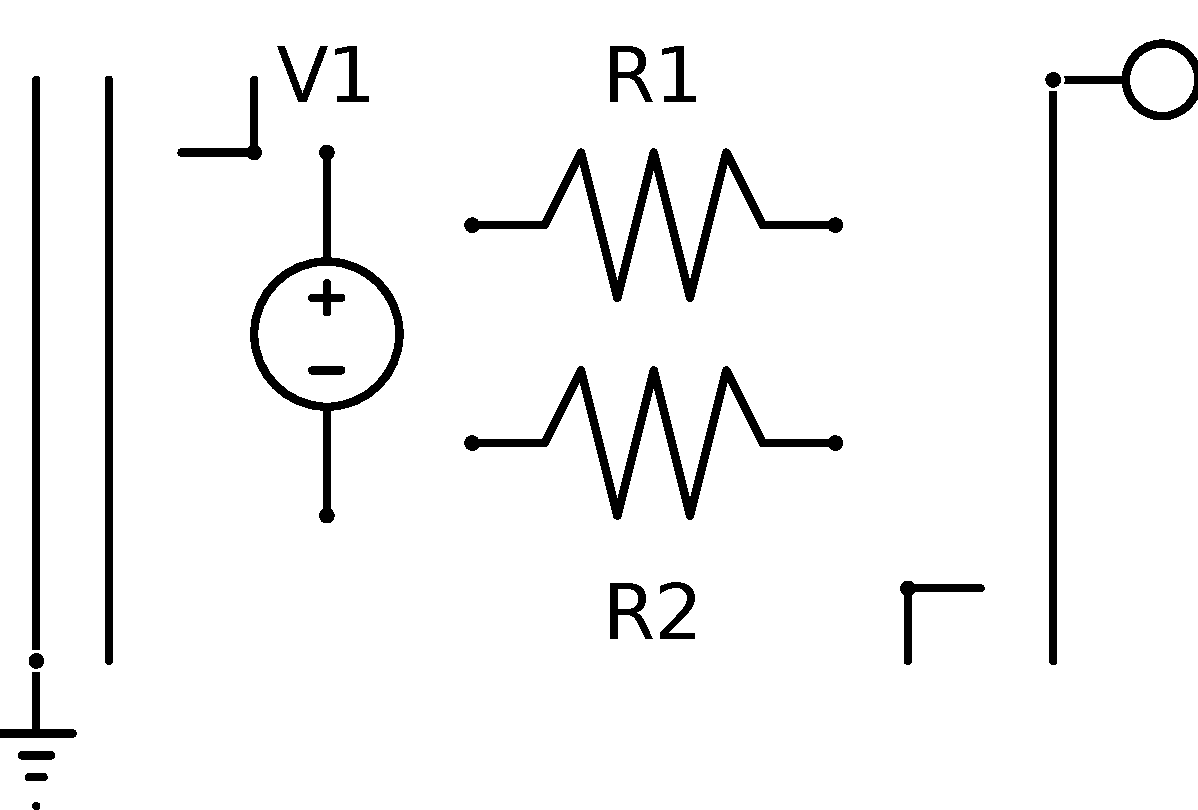
\includegraphics[scale=0.35]{immagini/design.pdf}
 \caption{Esempio di design per la ricostruzione}
 \label{cdes}
\end{figure}

La ricostruzione del circuito all'interno dell'ambiente di disegno avverrà sfruttando le diverse tipologie di fili disponibili, ovvero utilizzando ponticelli per la stesura dei collegamenti a partire dai componenti. Tali fili saranno diretti a punti di aggancio immediatamente esterni all'area occupata, dislocati sulla sinistra e sulla destra di essa, in numero bilanciato. Un'immagine che esemplifica quanto detto è riportata in figura \ref{cdes} dove, in particolare, è stato anche segnato il limite superiore-sinistro e inferiore-destro dello spazio occupato Il circuito è la ricostruzione di un divisore di tensione e i tre fili di riferimento possono essere assimilati a massa, tensione di uscita e punto di snodo fra il generatore e una delle due resistenze.

\paragraph{Il modello}
La descrizione del modello è svolta per passi, introducendo via via parametri e variabili e spiegandone il loro scopo e la loro utilità. Per una rappresentazione globale del modello utilizzato si faccia riferimento al listato \ref{allmod}. Si tenga presente che, per astrarre dal caso specifico, si sono separati il modello stesso dai dati, ottenendo così una rappresentazione generica del problema adattabile a qualsiasi situazione.

Il primo passo consiste nella definizione di un insieme che contenga i nostri componenti, identificabili per nome (così da facilitare le cose). Letteralmente:
\small
\begin{verbatim}
 set ITEM ;
\end{verbatim}
\normalsize
Il file dati potrebbe riportare molto semplicemente, ad esempio, nel caso del divisore di tensione in figura \ref{cdes}:
\small
\begin{verbatim}
 set ITEM := V1 R1 R2 ;
\end{verbatim}
\normalsize

A supporto dell'insieme dei componenti vi sono alcuni parametri su di esso definiti, per ogni elemento, ovvero larghezza e altezza dell'oggetto, oltre che il numero di nodi che devono tendere ad avvicinarsi al lato sinistro dello spazio occupato e il numero di nodi che viceversa devono tendere dal lato opposto (questo sarà strettamente dipendente dalla dislocazione dei punti di aggancio subito adiacenti all'area occupata). Infine, vi sarà un parametro che indicherà lo scostamento desiderato fra due componenti diversi, così da poter imporre una divisione a priori interna allo schema. Otteniamo:
\small
\begin{verbatim}
 param Width {i in ITEM} ;
 param Height {i in ITEM} ;
 param NL {i in ITEM} ;
 param NR {i in ITEM} ;
 param delta ;
\end{verbatim}
\normalsize
Sempre rifacendosi all'esempio del divisore di tensione, potremmo avere:
\small
\begin{verbatim}
 param Width :=
    V1 3
    R1 6
    R2 6
  ;

 param Height :=
    V1 6
    R1 3
    R2 3
  ;

 param NL :=
    V1 2
    R1 1
    R2 1
  ;

 param NR :=
    V1 0
    R1 1
    R2 1
  ;

 param delta := 1 ;
\end{verbatim}
\normalsize
Legando questi dati all'ambiente di disegno, si possono ricostruire nella direzione opposta alcune caratteristiche significative dei componenti.\\
Ad esempio, per quanto riguarda il generatore di tensione, si osserva che esso è rappresentato in posizione verticale ed ha un'occupazione di due celle in larghezza e cinque celle in altezza (ovvero tre separatori in larghezza racchiudono, evidentemente, due celle e in modo simile vale anche per l'altezza), mentre le resistenze sono disposte in posizione orizzontale, facilmente deducibile dai dati riguardanti l'area occupata.\\
In merito alle richieste sui nodi, le quali influiranno in seguito sul processo di dislocazione, si nota che il generatore di tensione ha una tendenza maggiore a spostarsi verso il lato sinistro dello spazio occupato (infatti, supponendo di avere tre nodi all'interno del circuito, il nodo massa e il primo snodo fra generatore e resistenza saranno posizionati sul lato sinistro dell'area occupata, pertanto necessariamente viene richiesta in questo caso una vicinanza a tale lato); in maniera simile le due resistenze sono entrambe connesse al terzo dei tre nodi presenti (posto a destra dello spazio occupato) e ad uno dei due nodi citati in precedenza, pertanto dividono le loro richieste fra i due lati dell'area occupata, mostrando una tendenza ad occupare posizioni centrali.\\
Si faccia riferimento alla figura \ref{vdiv_schema} per aiutare la comprensione dei dati.\\
L'ultimo parametro, \textit{delta}, indica banalmente un valore di discostamento che si desidera avere fra due componenti affiancati orizzontalmente o verticalmente. Vedremo come, in seguito, sarà utilizzato a tale scopo.

\begin{figure}[ht]
 \centering
 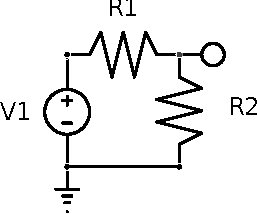
\includegraphics[scale=1]{immagini/vdiv_schema.pdf}
 \caption{Divisore di tensione}
 \label{vdiv_schema}
\end{figure}

Prima di dare una sommaria descrizione delle variabili utilizzate, è necessario soffermarsi in particolare su alcune di esse poiché coinvolte in un processo di sostituzione fra problemi equivalenti. In altri termini, senza discutere delle ripercussioni sull'intero modello, si osserva che una delle necessità principali è quella della riduzione dell'area occupata. Questa la si può esprimere come il perimetro definito dalla massima estensione in direzione orizzontale e in direzione verticale, ovvero sfruttando le posizioni dei componenti ($ \left( x, y\right) $, le quali sono nient'altro che alcuni dei valori che si mira ad ottenere) e la loro descrizione strutturale, può essere riassunta come:
$$ min \left(2 \ast \left(max_{i = 1\dots N}\{ x_i + width_i\} + max_{j = 1\dots N}\{ y_j + height_j\} \right)\right) $$
Inoltre, sebbene il modello non sia stato presentato ancora per intero, si può anticipare il fatto che vincoli contenenti ricerche sul massimo valore in ampiezza o altezza sono presenti anche in altri punti. Questo è, ovviamente, evitabile con pochi, semplici accorgimenti. Ancora, tralasciando i vincoli che in seguito coinvolgono gli stessi parametri, si può semplificare quanto sopra come segue:
\small
\begin{verbatim}
 var WDIM >= 0;
 var HDIM >= 0;
 var P = 2 * (WDIM + HDIM) ;
 var x {i in ITEM} >= 0, integer ;
 var y {i in ITEM} >= 0, integer ;

 minimize size: P ;

 subject to _supW {i in ITEM}: WDIM >= x[i] + Width[i] ;
 subject to _supH {i in ITEM}: HDIM >= y[i] + Height[i] ;
\end{verbatim}
\normalsize

Introducendo cioè due variabili che limitano superiormente l'estensione dell'area occupata si può facilmente dimostrare l'equivalenza dei due problemi, ottenendo di contro un miglioramento in termini di rappresentazione del problema. Procedendo, si aggiungono i vincoli relativi alle tendenze di accostamento verso uno dei lati dell'area occupata, le quali non necessitano di particolati approfondimenti, ovvero:
\small
\begin{verbatim}
minimize ldist: sum{i in ITEM} NL[i] * x[i] ;
minimize rdist: sum{i in ITEM} NR[i] * (WDIM - x[i] - Width[i]); 
\end{verbatim}
\normalsize

I due obiettivi sfruttano infatti la posizione dell'angolo superiore sinistro e superiore destro del componente per calcolare una distanza dai lati adiacenti ai punti di aggancio, quindi pesano tale distanza per le tendenze del componente e mirano ad ottenere un abbattimento globale che si sposi con la minimizzazione della superficie occupata.

Degno di nota è, invece, l'argomento delle posizioni relative fra componenti. Fino ad ora, infatti, si è sorvolato sul fatto che quest'ultimi non debbano sovrapporsi, condizione che però non si può rimandare a scapito del corretto comportamento del modello. Presi quindi due generici elementi, $i$ e $j$, si ha che il primo può trovarsi (relativamente alla posizione del secondo) sulla destra, sulla sinistra, in alto o in basso. Si noti inoltre che necessariamente \textbf{almeno uno di questi vincoli deve essere soddisfatto}.\\
Formalmente deve valere almeno uno fra i seguenti vincoli:
$$ x_i + width_i <= x_j~,~x_j + width_j <= x_i$$ $$y_i + height_i <= y_j~,~y_j + height_j <= y_i $$
Prendiamo in esame le componenti orizzontali. Si può introdurre una matrice quadrata $L \in \{0, 1\}^{N\ast N}$ (con $N$ numero di componenti nel circuito) tale per cui:
$$L_{ij} = 1 \Leftrightarrow x_i + width_i <= x_j $$
Similmente, si può imporre che per $T \in \{0, 1\}^{N\ast N}$:
$$T_{ij} = 1 \Leftrightarrow y_i + height_i <= y_j $$
La condizione esclusiva si trasforma quindi in:
$$ L_{ij} + L_{ji} + T_{ij} + T_{ji} >= 1 $$
Rimane da dare una forma alle singole condizioni. A tal proposito, senza perdere di generalità, prendiamo in esame $L_{ij}$. Necessariamente, questo deve valere $1$ laddove valga la condizione $ x_i + width_i <= x_j $. Otteniamo, pertanto:
$$ x_i + width_i - x_j <= 0\Rightarrow L_{ij} = 1~\rightarrow~L_{ij} = 0\Rightarrow x_i + width_i - x_j > 0 $$
$$\rightsquigarrow~x_i + width_i - x_j >= L_{i, j}\ast \left(- WDIM - delta\right) + delta $$
Dove si sfrutta il parametro \textit{delta} per imporre uno scostamento minimo fra due componenti dislocati uno di fianco all'altro. Ciò non basta, però, a soddisfare il vincolo esclusivo sulle posizioni relative. Bisogna infatti imporre anche la condizione opposta, ovvero:
$$ L_{ij} = 1\Rightarrow x_i + width_i - x_j <= 0~\rightarrow~x_i + width_i - x_j > 0\Rightarrow L_{ij} = 0 $$
$$\rightsquigarrow~x_i + width_i - x_j <= \left( 1 - L_{i, j}\right)\ast WDIM $$
Similmente vale per la situazione di posizione relativa verticale, per la quale otteniamo (in forma breve, tralasciando i calcoli in tutto e per tutto uguali ai precedenti):
$$ y_i + height_i - y_j >= T_{i, j}\ast \left(- HDIM - delta\right) + delta $$
$$ y_i + height_i - y_j <= \left( 1 - T_{i, j}\right)\ast HDIM $$

Quanto sopra, unito alla condizione esclusiva per le posizioni relative, è sufficiente a imporre che due componenti non si sovrappongano e al contempo riservino un margine minimo orizzontale e verticale (il quale, si deduce dalle espressioni sopra, è posto sulla destra e sul lato inferiore di ogni singolo componente, imponendo così anche uno scostamento alle estremità dell'area occupata).

Trascrivendo il tutto in formato coerente con quanto precedentemente illustrato, avremo:
\small
\begin{verbatim}
 var L {i in ITEM, j in ITEM}, binary ;
 var T {i in ITEM, j in ITEM}, binary ;

 subject to _L1 {i in ITEM, j in ITEM: j != i}:
   x[i] + Width[i] - x[j] <= (1 - L[i, j]) * WDIM ;
 subject to _L2 {i in ITEM, j in ITEM: j != i}:
   x[i] + Width[i] - x[j] >= L[i, j] * (- WDIM - delta) + delta ;
 subject to _T1 {i in ITEM, j in ITEM: j != i}:
   y[i] + Height[i] - y[j] <= (1 - T[i, j]) * HDIM ;
 subject to _T2 {i in ITEM, j in ITEM: j != i}:
   y[i] + Height[i] - y[j] >= T[i, j] * (- HDIM - delta) + delta ;

 subject to _ONCE {i in ITEM, j in ITEM: j != i}:
   L[i, j] + L[j, i] + T[i, j] + T[j, i] >= 1 ;
\end{verbatim}
\normalsize

Ricostruendo i vari pezzi, illustrati attraverso espressioni matematiche formali e con l'utilizzo del linguaggio AMPL \cite{ampl}, otteniamo infine il modello riportato nel listato \ref{allmod}.

\lstset{basicstyle=\small, language=, breaklines, breakatwhitespace}
\begin{lstlisting}[caption={Modello per floor-planning in sistemi CAD},float,captionpos=b,label=allmod,frame=lines]
set ITEM ;

param Width {i in ITEM} ;
param Height {i in ITEM} ;
param NL {i in ITEM} ;
param NR {i in ITEM} ;
param delta ;

var WDIM >= 0;
var HDIM >= 0;
var P = 2 * (WDIM + HDIM) ;
var x {i in ITEM} >= 0, integer ;
var y {i in ITEM} >= 0, integer ;

var L {i in ITEM, j in ITEM}, binary ;
var T {i in ITEM, j in ITEM}, binary ;


minimize size: P ;
minimize ldist: sum{i in ITEM} NL[i] * x[i] ;
minimize rdist: sum{i in ITEM} NR[i] * (WDIM - x[i] - Width[i]);

subject to _supW {i in ITEM}: WDIM >= x[i] + Width[i] ;
subject to _supH {i in ITEM}: HDIM >= y[i] + Height[i] ;

subject to _L1 {i in ITEM, j in ITEM: j != i}: x[i] + Width[i] - x[j] <= (1 - L[i, j]) * WDIM ;
subject to _L2 {i in ITEM, j in ITEM: j != i}: x[i] + Width[i] - x[j] >= L[i, j] * (- WDIM - delta) + delta ;
subject to _T1 {i in ITEM, j in ITEM: j != i}: y[i] + Height[i] - y[j] <= (1 - T[i, j]) * HDIM ;
subject to _T2 {i in ITEM, j in ITEM: j != i}: y[i] + Height[i] - y[j] >= T[i, j] * (- HDIM - delta) + delta ;

subject to _ONCE {i in ITEM, j in ITEM: j != i}: L[i, j] + L[j, i] + T[i, j] + T[j, i] >= 1 ;
\end{lstlisting}

\paragraph{Prove sperimentali}
Le prove sperimentali sono state effettuate utilizzando risolutori presenti sulla rete, o meglio direttamente accessibili dalla rete. Per la natura del problema era necessario sfruttare un risolutore che potesse approcciarsi con problematiche di programmazione intera non lineare, si è quindi pensato all'uso di \textit{Couenne} \cite{couenne} tramite il \textit{NEOS server} \cite{neos}\cite{neosserver}, ovvero l'utilizzo di risolutori specifici tramite interfacce web dalle quali fosse possibile sottomettere file di modello, dati e comandi in formato AMPL.

Per via della natura di accesso al risolutore sono state fatte alcune prove sperimentali su modelli relativamente piccoli di cui vi è una breve illustrazione in seguito.

\paragraph{Divisore di tensione}
\begin{figure}[ht]
 \centering
 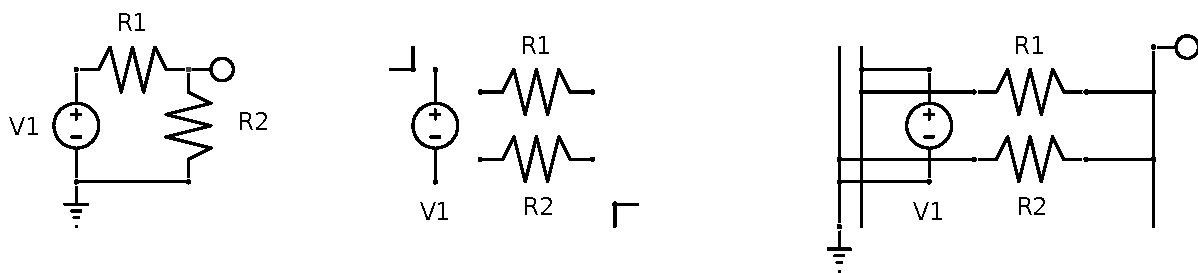
\includegraphics[scale=0.5]{immagini/voltage_divider.pdf}
 \caption{Divisore di tensione}
 \label{voltagedivider}
\end{figure}
Il primo modello è lo stesso utilizzato precedentemente per l'illustrazione di alcuni concetti chiave, ovvero il divisore di tensione riportato in figura \ref{voltagedivider}. Nella stessa immagine è riportato il modello di partenza, il modello adattato secondo i risultati ottenuti e la sua plausibile ricostruzione con l'aggiunta dei punti di aggancio e dei collegamenti necessari. I dati ricavati dall'esecuzione del risolutore sono riportati di seguito:
\small
\begin{verbatim}
 WDIM = 9
 HDIM = 6
 P = 30

 :    x   y    :=
 R1   3   0
 R2   3   3
 V1   0   0
 ;

 :       L   T    :=
 R1 R1   0   0
 R1 R2   0   1
 R1 V1   0   0
 R2 R1   0   0
 R2 R2   0   0
 R2 V1   0   0
 V1 R1   1   0
 V1 R2   1   0
 V1 V1   0   0
 ;
\end{verbatim}
\normalsize

\paragraph{Circuito RLC}
\begin{figure}[ht]
 \centering
 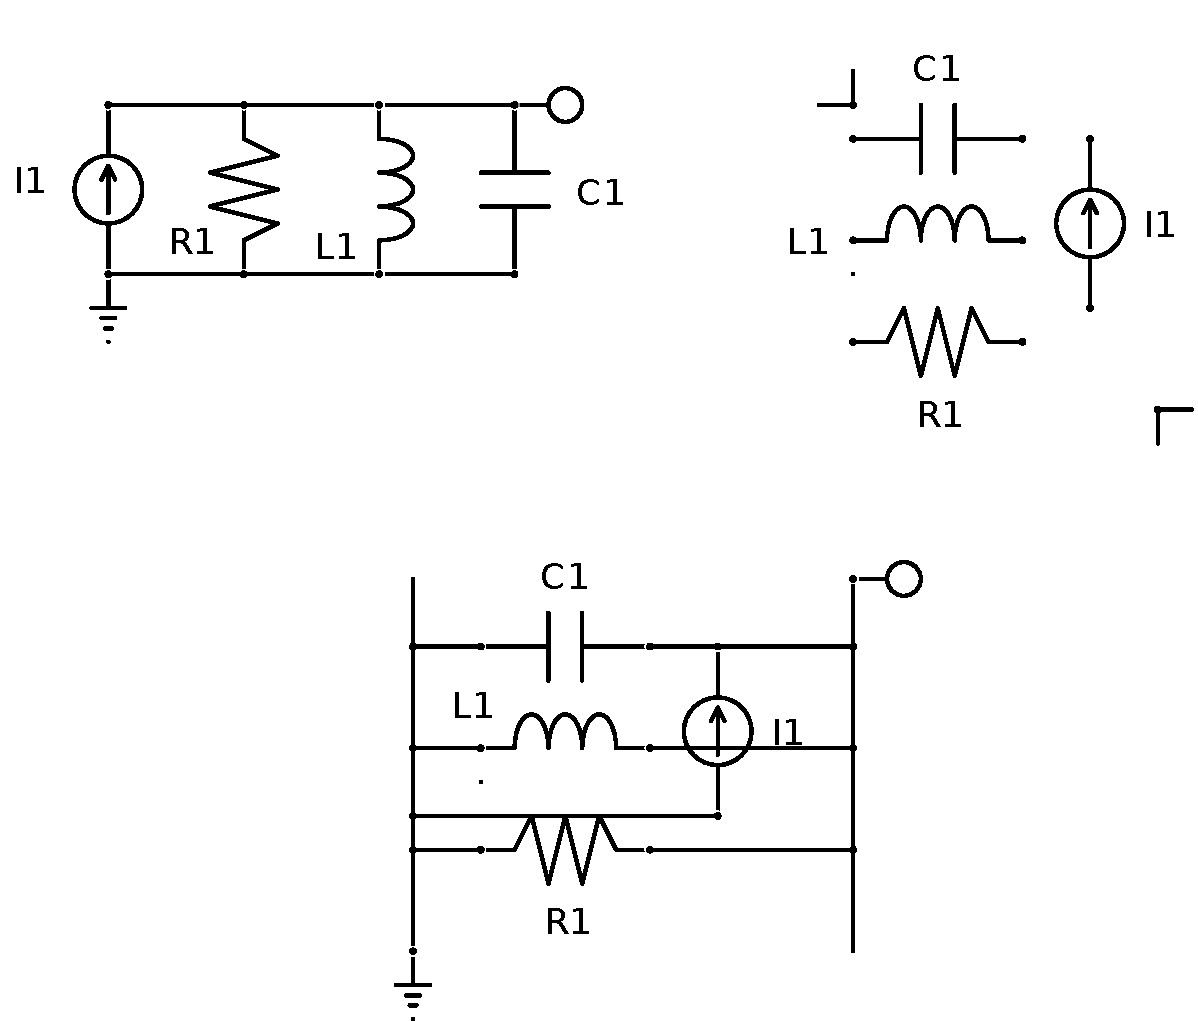
\includegraphics[scale=0.5]{immagini/rlc.pdf}
 \caption{Circuito RLC}
 \label{rlc}
\end{figure}
Un altro semplice modello adottato per le prove sprimentali è il circuito RLC. Senza indugiare oltre si osservi la figura \ref{rlc} che, come sopra, presenta il circuito originale, il circuito ricostruito e infine completato con i collegamenti necessari. I dati relativi a questo esempio sono i seguenti (per brevità, ci limitiamo a riportare le sole posizioni per quanto riguarda i dati ottenuti):
\small
\begin{verbatim}
 WDIM = 9
 HDIM = 9
 P = 36

 :    x   y    :=
 C1   0   0
 I1   6   1
 L1   0   3
 R1   0   6
 ;
\end{verbatim}
\normalsize
In questo caso si ha la sovrapposizione di alcuni collegamenti la quale, però, non comporta alcuna menomazione per il circuito finale.

\paragraph{Amplificatore invertente}
\begin{figure}[ht]
 \centering
 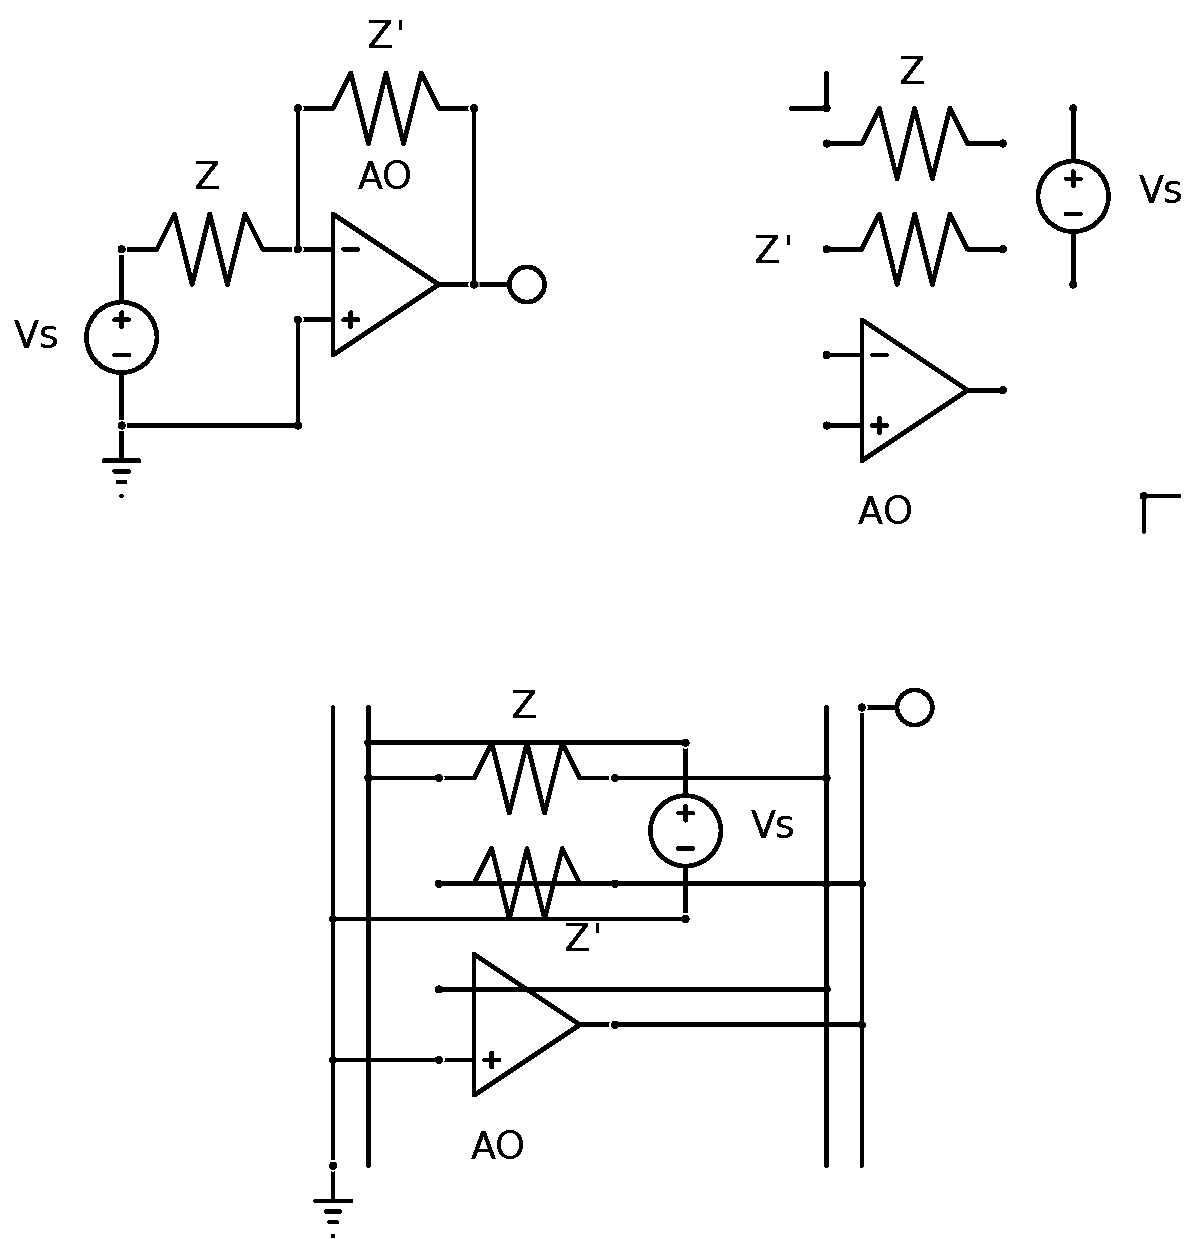
\includegraphics[scale=0.5]{immagini/amplinv.pdf}
 \caption{Amplificatore invertente}
 \label{amplinv}
\end{figure}
Cercando di svariare sulle forme dei componenti si è proposto un esempio che coinvolgesse un amplificatore operazionale, la cui forma è ben lungi dall'essere assimilabile a quella di generatori, resistenze e tutti gli altri componenti fino ad ora coinvolti. I risultati sono riportati in figura \ref{amplinv}:
\small
\begin{verbatim}
 WDIM = 9
 HDIM = 11
 P = 40

 :    x   y    :=
 AO   0   6
 Vs   6   0
 Z    0   0
 Z_   0   3
 ;
\end{verbatim}
\normalsize

\paragraph{Modello di amplificatore operazionale}
\begin{figure}[ht]
 \centering
 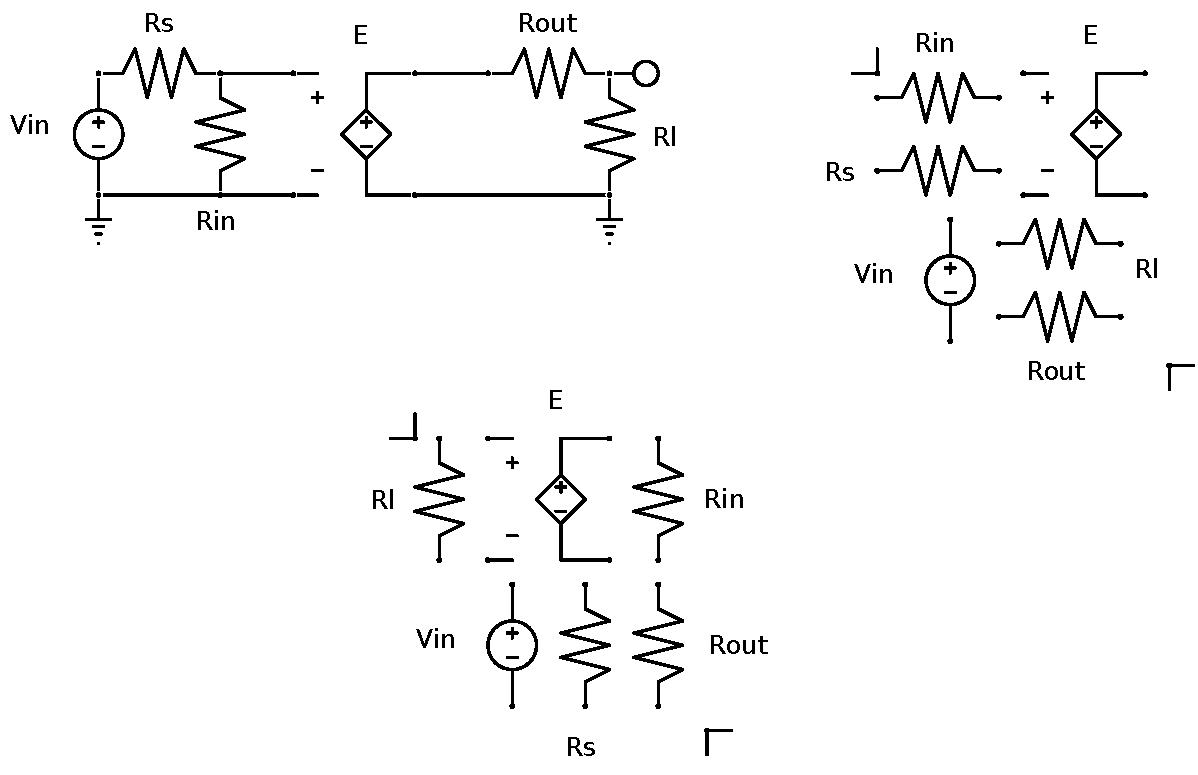
\includegraphics[scale=0.5]{immagini/ao.pdf}
 \caption{Amplificatore operazionale (modello)}
 \label{ao}
\end{figure}
L'ultimo esempio, leggermente più complesso in termini di numero di componenti, è il modello di un amplificatore operazionale espresso tramite resistenze e generatori controllati e non. In figura \ref{ao} i risultati ottenuti. In questo caso, come si può notare dalle figure, si è portato avanti un esperimento leggermente diverso dai precedenti, ovvero si è tentata una dislocazione secondo l'orientamento standard dei componenti e quindi, in un secondo momento, secondo una disposizione verticale di ogni componente. I risultati sono stati, ovviamente, diversi ma in entrambi i casi discreti e vicini per quanto riguarda la dimensione dell'area occupata.

\paragraph{Conclusioni}
La ricostruzione di un circuito elettrico a discapito delle informazioni semantiche ricavabili dai componenti coinvolti (procedimento che richiederebbe un'inaccessibile quantità di risorse di ogni genere) è un procedimento facilmente realizzabile con pochi vincoli, reso arduo esclusivamente dalla presenza di vincoli di interezza i quali complicano non poco il processo di risoluzione. Nel caso in esame, poi, una nota particolare va fatta ai vincoli di tendenza verso un lato specifico dell'area occupata: questi, infatti, non tengono conto della distribuzione dei punti di aggancio all'interno della superficie del componente e pertanto possono risultare se non superflui quanto meno utili più che altro ad appesantire il tutto. In fase di realizzazione, pertanto, potrebbe essere più conveniente sopprimere tali vincoli, snellendo il processo di risoluzione stesso e guadagnando inevitabilmente in termini di prestazioni, posizionando piuttosto il componente in modo intelligente, ovvero ad esempio sottoponendolo a rotazioni di $180^\circ$ affinché i punti di aggancio interni si avvicinino a quelli esterni. Inutile dire che per componenti con superificie quadrata la rotazione può anche essere arbitraria per multipli di $90^\circ$ mentre lo stesso non si può affermare per componenti con altezza e larghezza diverse.